\documentclass[11pt]{article}

\usepackage[utf8]{inputenc}
\usepackage[T1]{fontenc}
\usepackage{amsmath,amssymb}
\usepackage{graphicx}
\usepackage[margin=1in]{geometry}
\usepackage{booktabs}
\usepackage{siunitx}
\usepackage[super,square,comma]{natbib}
\usepackage{lineno}
\usepackage{xcolor}
\usepackage{hyperref}
\usepackage{tikz}
\usepackage{pgfplots}
\pgfplotsset{compat=1.18}

\linenumbers

\title{The Canonical Firefly Luminosity Is Overestimated by $10^3$--$10^4$-Fold}

\author{David H. Silver$^{1,*}$}

\date{}

\begin{document}

\maketitle

\noindent $^{1}$Remiza AI\\
$^{*}$Corresponding author: david@remiza.ai\\
ORCID: 0000-0002-3071-304X

\vspace{1em}

\begin{abstract}
The luminous intensity of \textit{Photinus pyralis} fireflies has been cited as 1/40 to 1/400 candlepower since the 1924 photometric study by Ives and Coblentz---a value corresponding to $3 \times 10^{13}$ to $3 \times 10^{14}$ photons per flash. We show that this canonical estimate exceeds the theoretical maximum imposed by luciferase abundance and quantum yield by $10^3$--$10^4$-fold. Direct field measurements with a calibrated lux meter yield $10^{10}$--$10^{11}$ photons per flash, consistent with both our biochemical bound and independent reanalysis of historical and modern spectroscopic data. The persistence of this error for a century reflects a disconnect between classical photometry and modern bioluminescence research, the latter reporting light output almost exclusively in arbitrary units rather than absolute photon flux.
\end{abstract}

\noindent\textbf{Keywords:} firefly bioluminescence; photometry; \textit{Photinus pyralis}; luciferase

%==============================================================================
\section{Introduction}
%==============================================================================

The commonly cited value for firefly brightness---``1/40 candlepower''---traces to early twentieth-century photometric studies by William Coblentz at the National Bureau of Standards. However, examination of the original sources reveals two compounding errors that have persisted for over a century.

Coblentz's 1912 Carnegie Institution monograph reports that flash measurements for \textit{Photinus pyralis} ranged from ``1/50 candle to 1/400 candle, the predominating values being 1/400 candle.''\cite{Coblentz1912} The measurements were acknowledged as difficult: ``Because of the inability to cause the insect to flash rapidly for any length of time, the measurements were more difficult, and hence uncertain.'' Specimens varied in brightness depending on whether they were freshly caught or had been in captivity; only about a dozen measurements were obtained from three healthy specimens. Despite this acknowledged uncertainty, subsequent authors appear to have either misread ``1/400'' as ``1/40'' (a transcription error) or cited the maximum value (1/50) while rounding to 1/40. The ``1/40 candlepower'' figure now appears in educational websites and textbooks, though Harvey's treatise\cite{Harvey1952} correctly cites Coblentz's range of ``1/50 to 1/400 candle.''

The problem with this number becomes apparent when one considers the molecular machinery responsible for firefly light production. The bioluminescent reaction is catalyzed by luciferase, a 62-kDa oxygenase encoded by the \textit{luc} gene, first cloned and sequenced in 1985.\cite{deWet1987} Luciferase catalyzes the adenylation of D-luciferin by ATP to form a luciferyl-adenylate intermediate, which is then oxidized by molecular oxygen to produce electronically excited oxyluciferin; relaxation to the ground state emits a photon at approximately 560 nm.\cite{Shimomura2006} Because each catalytic cycle consumes one luciferin molecule and produces at most one photon, the total light output of a flash is bounded by the product of the number of luciferase molecules in the lantern, the number of turnovers per enzyme during the flash, and the quantum yield of the reaction.

Estimates from histological cell counts and biochemical assays place the luciferase content of the firefly lantern at approximately $10^{11}$ molecules---roughly $10^5$ photocytes, each containing $10^6$ enzyme molecules at micromolar concentration.\cite{Viviani2002,Shimomura2006} The quantum yield has been precisely measured at 0.41, among the highest for any chemiluminescent system.\cite{Ando2008} Even under the most favorable kinetic assumptions, in which every enzyme molecule fires exactly once during the flash, the maximum possible output is $4 \times 10^{10}$ photons---four orders of magnitude below the canonical value.

This discrepancy appears to have gone unnoticed for nearly a century because the two relevant literatures rarely intersected. Following the classical photometric studies of the early twentieth century, bioluminescence research shifted toward molecular biology and biochemistry, with light output reported almost universally in ``arbitrary units'' (a.u.) or ``relative light units'' (RLU) rather than absolute photon counts---a practice that persists in contemporary studies of firefly flash behavior,\cite{Ohba2012,Ho2022} luciferase biochemistry,\cite{Branchini2005,Ugarova2005} and bioluminescence spectroscopy.\cite{Wood1989} We undertook to resolve this puzzle by measuring firefly flash brightness directly with a calibrated lux meter, deriving the theoretical bound from first principles, and reanalyzing historical and modern datasets that can be converted to absolute photon flux.


%==============================================================================
\section{Experimental}
%==============================================================================

\subsection{Theoretical framework}

The total photon output of a firefly flash can be expressed as the product of five factors, each independently constrained by experiment (Table~\ref{tab:parameters}): the number of photocytes $N_{\text{cells}}$ (dimensionless count), the number of luciferase molecules per photocyte $N_{\text{enz}}$ (molecules/cell), the effective turnover rate $k_{\text{eff}}$ (s$^{-1}$), the quantum yield $\Phi$ (photons/turnover, dimensionless), and the flash duration $t$ (s). Under steady-state conditions, $k_{\text{eff}} \approx 0.01$~s$^{-1}$ reflects oxygen-limited turnover in vivo.\cite{Timmins2001,Niwa2010} Under burst conditions, where the enzyme pool is pre-charged with substrate and discharged synchronously, each enzyme fires once ($n_{\text{turn}} = 1$). Three scenarios span the plausible range:
\begin{align}
N_\gamma^{\text{(min)}} &= \underbrace{10^5}_{N_{\text{cells}}} \times \underbrace{10^6}_{N_{\text{enz}}} \times \underbrace{0.01}_{k_{\text{eff}}} \times \underbrace{0.41}_{\Phi} \times \underbrace{0.25}_{t} = 10^8 \text{ photons} \\[6pt]
N_\gamma^{\text{(mid)}} &= 10^5 \times 10^6 \times 0.1\phantom{0} \times 0.41 \times 0.25 = 10^9 \text{ photons} \\[6pt]
N_\gamma^{\text{(max)}} &= 10^5 \times 10^6 \times \underbrace{1\phantom{.00}}_{\text{burst}} \times 0.41 \times 1\phantom{.00} = 4 \times 10^{10} \text{ photons}
\end{align}

\begin{table}[htbp]
\centering
\caption{Biochemical parameters constraining firefly photon output. Each parameter is independently bounded; the product yields the theoretical photon range.}
\label{tab:parameters}
\small
\begin{tabular}{@{}lccccm{5.5cm}@{}}
\toprule
Parameter & Symbol & Min & Mid & Max & Constraint basis \\
\midrule
Photocytes & $N_{\text{cells}}$ & $10^5$ & $10^5$ & $10^5$ & Histological counts in \textit{P.\ pyralis}\cite{Viviani2002} \\[6pt]
Enzymes/cell & $N_{\text{enz}}$ & $10^6$ & $10^6$ & $10^6$ & $\mu$M luciferase in photocytes\cite{Shimomura2006} \\[6pt]
Turnover (s$^{-1}$) & $k_{\text{eff}}$ & 0.01 & 0.1 & 1 & O$_2$-limited (min) to burst kinetics (max)\cite{Timmins2001} \\[6pt]
Quantum yield & $\Phi$ & 0.41 & 0.48 & 0.88 & pH-dependent; 0.41--0.88 reported\cite{Ando2008,Shimomura2006} \\[6pt]
Duration (s) & $t$ & 0.25 & 0.25 & 1 & Flash 200--300~ms; burst fires once\cite{Lewis2008} \\
\midrule
\textbf{Product} & $N_\gamma$ & $\mathbf{10^8}$ & $\mathbf{10^9}$ & $\mathbf{4 \times 10^{10}}$ & Equations 1--3 \\
\bottomrule
\end{tabular}
\end{table}

\subsection{Photometric units and conversions}

Comparing historical and modern light measurements requires careful attention to units. Photometric units weight radiant power by human visual sensitivity, while radiometric units measure absolute power. Table~\ref{tab:units} summarizes the key quantities.

\begin{table}[h]
\centering
\small
\caption{Photometric and radiometric quantities.}
\label{tab:units}
\begin{tabular}{@{}llll@{}}
\toprule
Quantity & Symbol & Unit & Definition \\
\midrule
Radiant power & $\Phi_e$ & W & Energy per unit time \\
Photon rate & $\dot{N}$ & s$^{-1}$ & $\Phi_e / E_\gamma$ where $E_\gamma = hc/\lambda$ \\
\midrule
Luminous intensity & $I_v$ & cd & Power per solid angle, weighted by $V(\lambda)$ \\
Luminous flux & $\Phi_v$ & lm & Total luminous power; $\Phi_v = 4\pi I_v$ (isotropic) \\
Illuminance & $E$ & lux (lm/m$^2$) & Flux per unit area; $E = I_v/r^2$ \\
Luminance & $L$ & cd/m$^2$ & Intensity per unit emitting area \\
\bottomrule
\end{tabular}
\end{table}

The conversion between systems uses the luminous efficacy $K_m = 683$~lm/W at peak photopic sensitivity (555~nm) and the luminosity function $V(\lambda)$:
\begin{equation}
\Phi_e = \frac{\Phi_v}{K_m \, V(\lambda)}, \qquad
\dot{N} = \frac{\Phi_e}{E_\gamma} = \frac{\Phi_v \, \lambda}{K_m \, V(\lambda) \, hc}
\label{eq:conversion}
\end{equation}
For firefly emission at $\lambda = 560$~nm, $V(\lambda) \approx 0.995$ and $E_\gamma = 3.55 \times 10^{-19}$~J, so photometric and radiometric measures nearly coincide. One lux at 560~nm corresponds to $2.6 \times 10^{12}$~photons$\cdot$s$^{-1}\cdot$m$^{-2}$.

The historical unit \textit{candlepower} is approximately equal to one candela, but early standards (the ``standard candle,'' Hefner lamp, and Carcel lamp) differed by up to 10\%, and one \textit{lambert} equals $(1/\pi) \times 10^4$~cd/m$^2$.

\subsection{Field measurements}

Flash illuminance was measured in Sungai Petani, Kedah, Malaysia, in November 2025, using wild-caught fireflies (likely \textit{Pteroptyx} species). A digital lux meter (0.1-lux resolution, $\pm$4\% accuracy, 2 Hz sampling) was positioned at 1--5 cm from the lantern of individually isolated fireflies in transparent containers. Ambient illumination was confirmed at 0.0 lux before each trial; a reference LED was measured nightly to verify instrument stability, and reported $\sim4.2$ lux before each measurement. Results are summarized in Table~\ref{tab:luxdata}.

\begin{table}[htbp]
\centering
\caption{Field lux-meter measurements (Sungai Petani, Malaysia, November 2025; $n=5$ fireflies).}
\label{tab:luxdata}
\begin{tabular}{lccc}
\toprule
Distance & Mean $\Delta$Lux & Max $\Delta$Lux & Flashes \\
\midrule
1 cm & 0.30 & 0.5 & 10 \\
2 cm & 0.23 & 0.5 & 10 \\
3 cm & 0.04 & 0.2 & 10 \\
4 cm & 0.04 & 0.2 & 8 \\
5 cm & 0.03 & 0.2 & 10 \\
\bottomrule
\end{tabular}
\end{table}

\subsection{Photometric conversion}

Illuminance $E$ (lux) at distance $r$ was converted to photon emission rate using:
\[
\dot{N} = \frac{4\pi E r^2}{K_m \, V(\lambda) \, E_\gamma}
\]
where $K_m = 683$ lm/W, $V(560\text{ nm}) = 0.995$, and $E_\gamma = hc/\lambda = 3.55 \times 10^{-19}$ J. This formula assumes isotropic (4$\pi$ sr) emission. However, firefly lanterns emit directionally: the photocyte layer sits beneath a dorsal reflector of uric acid crystals that backscatters upward-directed photons, channeling most light ventrally into a solid angle of approximately 1--2 sr (Figure~\ref{fig:geometry}).\cite{Bay2012} A geometric correction factor $f_{\text{geom}} = \Omega_{\text{eff}}/4\pi \approx 0.08$--$0.16$ was therefore applied.

\subsection{Reanalysis of published data}

Published measurements from Harvey \& Stevens (1928)\cite{Harvey1928} and Goh \& Wang (2022)\cite{Goh2022} were converted to photon flux using the same photometric framework. Harvey \& Stevens reported surface brightness of \textit{Pyrophorus} click-beetle lanterns (0.045 lambert over ${\sim}1$ mm$^2$); Goh \& Wang reported spectral irradiance of \textit{Photinus} flashes measured by fiber-optic spectrometry.


%==============================================================================
\section{Results}
%==============================================================================

Peak flash illuminance ranged from 0.2 to 0.5 lux at 1--2 cm distance (Table~\ref{tab:luxdata}), with weaker signals at greater distances following the expected inverse-square falloff. For the strongest flashes (0.5 lux at 1 cm), the isotropic calculation yields $\dot{N} \approx 10^{13}$ photons/s. Applying the geometric correction ($f_{\text{geom}} = 0.08$--$0.16$) and integrating over a 250-ms flash duration gives:
\[
N_\gamma = 10^{10}\text{--}4 \times 10^{11} \text{ photons per flash}
\]

This range is consistent with the theoretical bound ($10^8$--$4 \times 10^{10}$) and lies three to four orders of magnitude below the canonical 1924 value.

Two independent datasets corroborate this result (Table~\ref{tab:comparison}, Figure~\ref{fig:comparison}). Conversion of the Harvey \& Stevens (1928) surface brightness measurement yields ${\sim}6 \times 10^{11}$ photons per flash for the larger \textit{Pyrophorus} lanterns. Goh et al.\ (2022) measured luminescent intensity of nine Taiwanese firefly species at 1.2--14~lux for males and 0.8--5.8~lux for females (182--2048~nW/cm$^2$ and 123--850~nW/cm$^2$, respectively);\cite{Goh2022} assuming close-range measurement (${\sim}5$~cm) and applying our photometric conversion with geometric correction, these values correspond to $10^{10}$--$10^{11}$ photons per flash.

\begin{table}[htbp]
\centering
\caption{Photon emission estimates from independent sources.}
\label{tab:comparison}
\begin{tabular}{llcc}
\toprule
Source & Method & Reported value & Photons/flash \\
\midrule
Commonly cited & ``1/40 candle'' & 0.025 cd & $3 \times 10^{14}$ \\
Coblentz (1912) original$^\dagger$ & Visual photometry & 1/400 candle & $3 \times 10^{13}$ \\
Harvey \& Stevens (1928)$^*$ & Surface brightness & 45 mL & $6 \times 10^{11}$ \\
Goh et al.\ (2022)$^*$ & Lux meter & 1--14 lux & $10^{10}$--$10^{11}$ \\
Biochemical bound & Enzyme $\times$ yield & --- & $10^8$--$4 \times 10^{10}$ \\
This work & Lux meter & 0.2--0.5 lux & $10^{10}$--$4 \times 10^{11}$ \\
\bottomrule
\multicolumn{4}{l}{\footnotesize $^\dagger$``Predominating values'' per original text; range was 1/50--1/400 candle.}\\
\multicolumn{4}{l}{\footnotesize $^*$Our conversion of published data to photon flux.}
\end{tabular}
\end{table}

Indirect support comes from the in vitro quantum yield measurements of Ando et al.\ (2008), who reacted $2.98 \times 10^{11}$ luciferin molecules with excess luciferase and obtained ${\sim}10^{11}$ total photons (their Fig.\ 1a), confirming that the quantum yield of ${\sim}0.41$ holds at the absolute scale.\cite{Ando2008} This validates our biochemical bound: if the lantern contains ${\sim}10^{11}$ luciferase molecules and each fires once, the maximum output is ${\sim}4 \times 10^{10}$ photons---not $10^{14}$.

All four independent estimates---our lux-meter measurements, the biochemical bound, and the two converted datasets---converge on $10^{10}$--$10^{11}$ photons per flash. The 1924 Ives and Coblentz value ($3 \times 10^{14}$) stands alone as an outlier by $10^3$--$10^4$.

\begin{figure}[htbp]
\centering
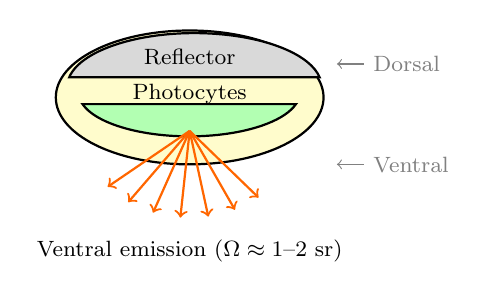
\begin{tikzpicture}[scale=0.85]
    \draw[thick, fill=yellow!20] (0,0) ellipse (2cm and 1cm);
    \draw[thick, fill=gray!30] (-1.8,0.3) arc (170:10:1.9cm and 0.8cm) -- (1.8,0.3) -- cycle;
    \node[font=\footnotesize] at (0,0.6) {Reflector};
    \draw[thick, fill=green!30] (-1.6,-0.1) arc (195:345:1.65cm and 0.65cm) -- cycle;
    \node[font=\footnotesize] at (0,0.05) {Photocytes};
    \foreach \angle in {-50,-35,-20,-5,10,25,40} {
        \draw[->, orange!80!red, thick] (0,-0.5) -- ({1.6*sin(\angle)},{-0.5-1.3*cos(\angle)});
    }
    \node[font=\footnotesize] at (0,-2.3) {Ventral emission ($\Omega \approx 1$--2 sr)};
    \draw[<-, gray] (2.2,0.5) -- (2.6,0.5) node[right, font=\footnotesize] {Dorsal};
    \draw[<-, gray] (2.2,-1.0) -- (2.6,-1.0) node[right, font=\footnotesize] {Ventral};
\end{tikzpicture}
\caption{Cross-section of the firefly lantern. The dorsal uric-acid reflector restricts emission to approximately 1--2 steradians; calculations assuming isotropic emission ($4\pi$ sr) overestimate total photon flux by a factor of 6--12.}
\label{fig:geometry}
\end{figure}

\begin{figure}[htbp]
\centering
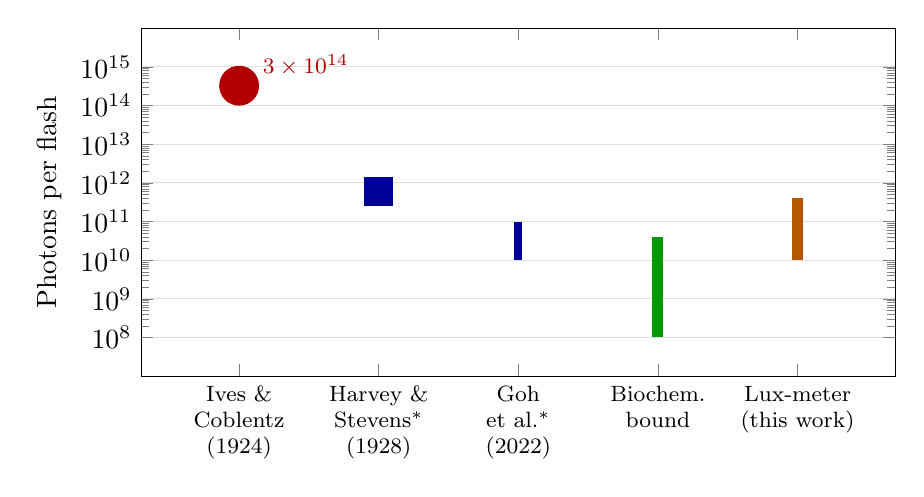
\begin{tikzpicture}
\begin{semilogyaxis}[
    width=0.92\textwidth,
    height=6cm,
    ylabel={Photons per flash},
    ymin=1e7, ymax=1e16,
    ytick={1e8,1e9,1e10,1e11,1e12,1e13,1e14,1e15},
    xtick={1,2,3,4,5},
    xticklabels={{Ives \&\\Coblentz\\(1924)},{Harvey \&\\Stevens$^*$\\(1928)},{Goh\\et al.$^*$\\(2022)},{Biochem.\\bound},{Lux-meter\\(this work)}},
    xticklabel style={align=center, font=\footnotesize},
    xmin=0.3, xmax=5.7,
    ymajorgrids=true,
    grid style={gray!25},
]
\addplot[only marks, mark=*, mark size=7pt, red!70!black] coordinates {(1, 3.26e14)};
\node[red!70!black, font=\footnotesize, anchor=south west] at (axis cs:1.1,3.26e14) {$3 \times 10^{14}$};
\addplot[only marks, mark=square*, mark size=5pt, blue!60!black] coordinates {(2, 6e11)};
\draw[blue!60!black, line width=3pt] (axis cs:3,1e10) -- (axis cs:3,1e11);
\draw[green!60!black, line width=4pt] (axis cs:4,1e8) -- (axis cs:4,4e10);
\draw[orange!70!black, line width=4pt] (axis cs:5,1e10) -- (axis cs:5,4e11);
\end{semilogyaxis}
\end{tikzpicture}
\caption{Photon emission estimates from independent sources. The 1924 value (red) is an outlier by $10^3$--$10^4$; all other estimates converge on $10^{10}$--$10^{11}$ photons per flash. $^*$Our conversion of published data.}
\label{fig:comparison}
\end{figure}


%==============================================================================
\section{Discussion}
%==============================================================================

The canonical firefly luminosity value is incorrect by three to four orders of magnitude, and two distinct errors appear to have compounded over the past century.

\textbf{Error 1: Transcription or rounding.} Coblentz's original 1912 data clearly state that the predominant flash intensity was 1/400 candle, with a maximum of 1/50 candle.\cite{Coblentz1912} Harvey's treatise\cite{Harvey1952} correctly cites this range (``1/50 to 1/400 candle''), yet the value propagated through secondary literature is ``1/40 candle''---either a transcription error (1/400 $\to$ 1/40) or a rounded maximum (1/50 $\approx$ 1/40). The erroneous figure appears in educational websites, textbooks, and even a University of Florida compendium that cites ``1/50 that of a sperm candle'' as the \textit{greatest} recorded intensity for \textit{Photinus pyralis}.\cite{Levy1998}

\textbf{Error 2: Methodological biases.} Even accepting 1/400 candle as the original measurement, Coblentz's visual nulling photometry introduces several systematic biases when applied to brief, spectrally narrow emissions: (1) observers tend to match peak rather than time-integrated intensity, inflating the estimate by a factor of 2--4; (2) the candlepower unit assumes isotropic emission, whereas firefly lanterns emit directionally into 1--2 steradians, inflating the estimate by a factor of 6--12; (3) firefly emission peaks at 560 nm, precisely at maximum human photopic sensitivity, potentially causing spectral mismatch relative to broadband reference lamps; and (4) calibration against the Hefner lamp standard carried approximately 20\% uncertainty. These biases multiply rather than add.

\textbf{Corroborating historical data.} Harvey \& Stevens (1928) measured the surface brightness of \textit{Pyrophorus} click-beetle lanterns at 45 millilamberts over a 1 mm$^2$ area.\cite{Harvey1928,Levy1998} Converting this to photon flux yields ${\sim}6 \times 10^{11}$ photons per flash---consistent with our measurements and far below the canonical value. Langley and Very's (1890) earlier measurements of \textit{Pyrophorus noctilucus} gave 1/1600 candle, also orders of magnitude below the commonly cited firefly value.\cite{Langley1890,Coblentz1912}

\textbf{Persistence of the error.} The separation between classical photometry and modern bioluminescence research allowed this error to persist unchallenged. Lynn Faust, author of \textit{Fireflies, Glow-worms, and Lightning Bugs}, notes that fireflies appear far brighter to the naked eye than to cameras because their emission sits at peak human photopic sensitivity of 555 nm (personal communication). This perceptual amplification may have contributed to the original overestimate, and the subsequent shift toward arbitrary-unit reporting in biochemical studies meant the discrepancy was never confronted directly.

Four independent lines of evidence---our lux-meter measurements, the converted Harvey \& Stevens data, the converted Goh \& Wang spectrometry, and the theoretical biochemical bound---all converge on $10^{10}$--$10^{11}$ photons per flash. This should replace the erroneous value in future references.


%==============================================================================
\section*{Acknowledgments}
%==============================================================================

Muhammad Naqiudeen Yunus (Sungai Petani, Malaysia) conducted the field lux-meter measurements.

We reached out to bioluminescence experts. Dr.\ Timothy R.\ Fallon, a scholar at Scripps Institution of Oceanography studying firefly photobiology, kindly granted permission to be cited (personal communication, Mar 4, 2025). His working estimate for a \textit{Photinus pyralis} flash was $10^8$--$10^9$ photons total per flash---consistent with our biochemical model and significantly below the canonical value. Lynn Faust offered the key insight that fireflies appear far dimmer to camera sensors than to the naked eye.

\section*{Data Availability}
Raw lux-meter data are available from the corresponding author on request.

%==============================================================================
\bibliographystyle{unsrtnat}
\bibliography{references}

\end{document}
